\chapter{迁移学习}\label{ux7b2cux5341ux4e00ux7ae0-ux8fc1ux79fbux5b66ux4e60}

​
本章主要简明地介绍了迁移学习的基本概念、迁移学习的必要性、研究领域和基本方法。重点介绍了几大类常用的迁移学习方法:数据分布自适应方法、特征选择方法、子空间学习方法、以及目前最热门的深度迁移学习方法。除此之外,我们也结合最近的一些研究成果对未来迁移学习进行了一些展望。并提供了一些迁移学习领域的常用学习资源,以方便感兴趣的读者快速开始学习。

\section{迁移学习基础知识}\label{ux8fc1ux79fbux5b66ux4e60ux57faux7840ux77e5ux8bc6}

\subsection{什么是迁移学习?}\label{ux4ec0ux4e48ux662fux8fc1ux79fbux5b66ux4e60}

找到目标问题的相似性,迁移学习任务就是从相似性出发,将旧领域(domain)学习过的模型应用在新领域上。

\subsection{为什么需要迁移学习?}\label{ux4e3aux4ec0ux4e48ux9700ux8981ux8fc1ux79fbux5b66ux4e60}

\begin{enumerate}
\def\labelenumi{\arabic{enumi}.}
\tightlist
\item
  \textbf{大数据与少标注的矛盾}:虽然有大量的数据,但往往都是没有标注的,无法训练机器学习模型。人工进行数据标定太耗时。
\item
  \textbf{大数据与弱计算的矛盾}:普通人无法拥有庞大的数据量与计算资源。因此需要借助于模型的迁移。
\item
  \textbf{普适化模型与个性化需求的矛盾}:即使是在同一个任务上,一个模型也往往难以满足每个人的个性化需求,比如特定的隐私设置。这就需要在不同人之间做模型的适配。
\item
  \textbf{特定应用(如冷启动)的需求}。
\end{enumerate}

\subsection{迁移学习的基本问题有哪些?}\label{ux8fc1ux79fbux5b66ux4e60ux7684ux57faux672cux95eeux9898ux6709ux54eaux4e9b}

基本问题主要有3个:

\begin{itemize}
\tightlist
\item
  \textbf{How to transfer}: 如何进行迁移学习?(设计迁移方法)
\item
  \textbf{What to transfer}:
  给定一个目标领域,如何找到相对应的源领域,然后进行迁移?(源领域选择)
\item
  \textbf{When to transfer}:
  什么时候可以进行迁移,什么时候不可以?(避免负迁移)
\end{itemize}

\subsection{迁移学习有哪些常用概念?}\label{ux8fc1ux79fbux5b66ux4e60ux6709ux54eaux4e9bux5e38ux7528ux6982ux5ff5}

\begin{itemize}
\tightlist
\item
  基本定义
\item
  \textbf{域(Domain)}:数据特征和特征分布组成,是学习的主体

  \begin{itemize}
  \tightlist
  \item
    \textbf{源域 (Source domain)}:已有知识的域
  \item
    \textbf{目标域 (Target domain)}:要进行学习的域
  \end{itemize}
\item
  \textbf{任务 (Task)}:由目标函数和学习结果组成,是学习的结果
\item
  按特征空间分类
\item
  \textbf{同构迁移学习(Homogeneous TL)}:
  源域和目标域的特征空间相同,\(D_s=D_t\)
\item
  \textbf{异构迁移学习(Heterogeneous
  TL)}:源域和目标域的特征空间不同,\(D_s\ne D_t\)
\item
  按迁移情景分类
\item
  \textbf{归纳式迁移学习(Inductive TL)}:源域和目标域的学习任务不同
\item
  \textbf{直推式迁移学习(Transductive
  TL)}:源域和目标域不同,学习任务相同
\item
  \textbf{无监督迁移学习(Unsupervised TL)}:源域和目标域均没有标签
\item
  按迁移方法分类
\item
  \textbf{基于实例的迁移 (Instance based
  TL)}:通过权重重用源域和目标域的样例进行迁移
\item
  \textbf{基于特征的迁移 (Feature based
  TL)}:将源域和目标域的特征变换到相同空间
\item
  \textbf{基于模型的迁移 (Parameter based
  TL)}:利用源域和目标域的参数共享模型
\item
  \textbf{基于关系的迁移 (Relation based
  TL)}:利用源域中的逻辑网络关系进行迁移
\end{itemize}

\begin{figure}
\centering
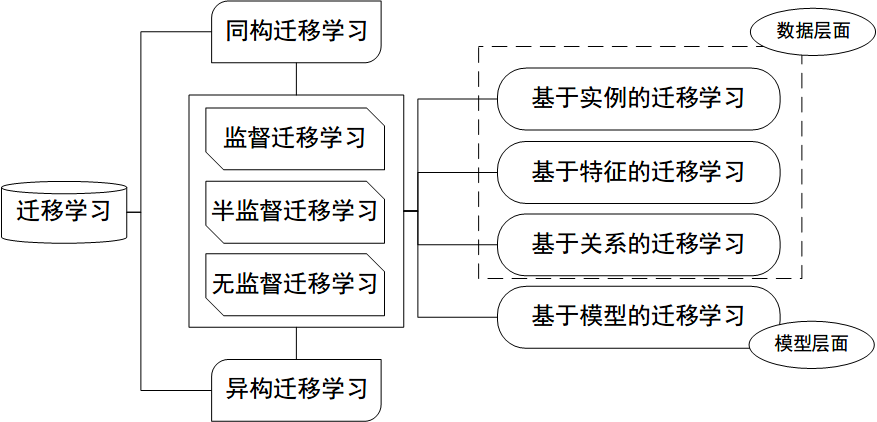
\includegraphics{./img/ch11/1542972502781.png}
\caption{1542972502781}
\end{figure}

\begin{figure}
\centering
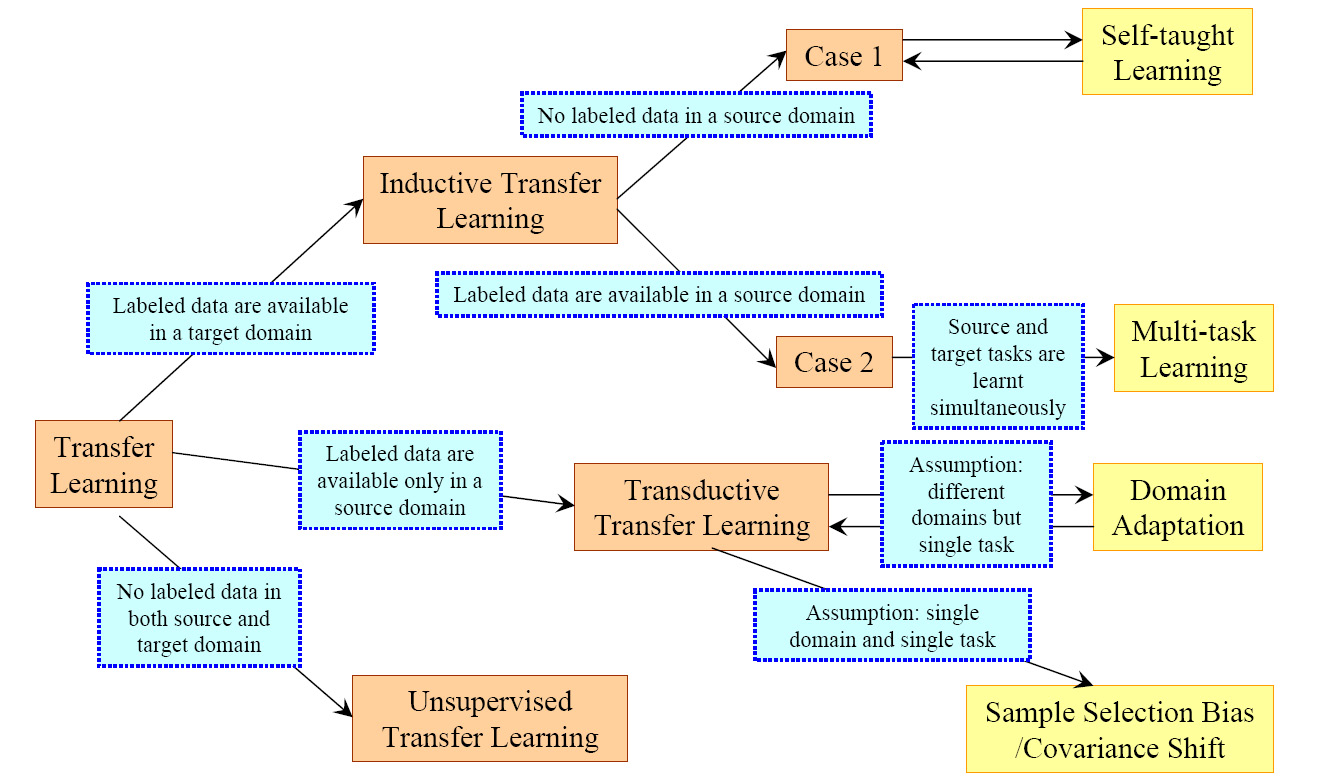
\includegraphics{./img/ch11/1542974131814.png}
\caption{1542974131814}
\end{figure}

\subsection{迁移学习与传统机器学习有什么区别?}\label{ux8fc1ux79fbux5b66ux4e60ux4e0eux4f20ux7edfux673aux5668ux5b66ux4e60ux6709ux4ec0ux4e48ux533aux522b}

\begin{longtable}[]{@{}lll@{}}
\toprule
& 迁移学习 & 传统机器学习\tabularnewline
\midrule
\endhead
数据分布 & 训练和测试数据不需要同分布 &
训练和测试数据同分布\tabularnewline
数据标签 & 不需要足够的数据标注 & 足够的数据标注\tabularnewline
建模 & 可以重用之前的模型 & 每个任务分别建模\tabularnewline
\bottomrule
\end{longtable}

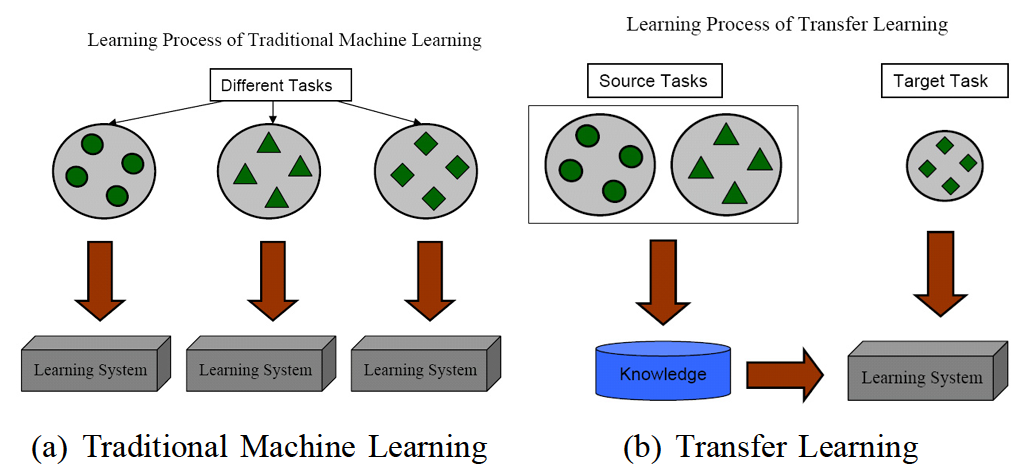
\includegraphics{./img/ch11/1542973960796.png} \#\#\# 11.1.6
迁移学习的核心及度量准则?

\textbf{迁移学习的总体思路可以概括为}:开发算法来最大限度地利用有标注的领域的知识,来辅助目标领域的知识获取和学习。

\textbf{迁移学习的核心是}:找到源领域和目标领域之间的相似性,并加以合理利用。这种相似性非常普遍。比如,不同人的身体构造是相似的;自行车和摩托车的骑行方式是相似的;国际象棋和中国象棋是相似的;羽毛球和网球的打球方式是相似的。这种相似性也可以理解为不变量。以不变应万变,才能立于不败之地。

\textbf{有了这种相似性后,下一步工作就是,
如何度量和利用这种相似性。}度量工作的目标有两点:一是很好地度量两个领域的相似性,不仅定性地告诉我们它们是否相似,更定量地给出相似程度。二是以度量为准则,通过我们所要采用的学习手段,增大两个领域之间的相似性,从而完成迁移学习。

\textbf{一句话总结: 相似性是核心,度量准则是重要手段。}

\subsection{迁移学习与其他概念的区别?}\label{ux8fc1ux79fbux5b66ux4e60ux4e0eux5176ux4ed6ux6982ux5ff5ux7684ux533aux522b}

\begin{enumerate}
\def\labelenumi{\arabic{enumi}.}
\tightlist
\item
  迁移学习与多任务学习关系:
\end{enumerate}

\begin{itemize}
\tightlist
\item
  \textbf{多任务学习}:多个相关任务一起协同学习;
\item
  \textbf{迁移学习}:强调信息复用,从一个领域(domain)迁移到另一个领域。
\end{itemize}

\begin{enumerate}
\def\labelenumi{\arabic{enumi}.}
\setcounter{enumi}{1}
\tightlist
\item
  迁移学习与领域自适应:\textbf{领域自适应}:使两个特征分布不一致的domain一致。
\item
  迁移学习与协方差漂移:\textbf{协方差漂移}:数据的条件概率分布发生变化。
\end{enumerate}

Reference:

\begin{enumerate}
\def\labelenumi{\arabic{enumi}.}
\tightlist
\item
  \href{https://github.com/jindongwang/transferlearning-tutorial}{王晋东,迁移学习简明手册}
\item
  Ben-David, S., Blitzer, J., Crammer, K., Kulesza, A., Pereira, F., \&
  Vaughan, J. W. (2010). A theory of learning from different domains.
  Machine learning, 79(1-2), 151-175.
\item
  Tan, B., Song, Y., Zhong, E. and Yang, Q., 2015, August. Transitive
  transfer learning. In Proceedings of the 21th ACM SIGKDD International
  Conference on Knowledge Discovery and Data Mining (pp.~1155-1164).
  ACM.
\end{enumerate}

\subsection{什么是负迁移?产生负迁移的原因有哪些?}\label{ux4ec0ux4e48ux662fux8d1fux8fc1ux79fbux4ea7ux751fux8d1fux8fc1ux79fbux7684ux539fux56e0ux6709ux54eaux4e9b}

负迁移(Negative
Transfer)指的是,在源域上学习到的知识,对于目标域上的学习产生负面作用。

产生负迁移的原因主要有: - 数据问题:源域和目标域压根不相似,谈何迁移?
-
方法问题:源域和目标域是相似的,但是,迁移学习方法不够好,没找到可迁移的成分。

负迁移给迁移学习的研究和应用带来了负面影响。在实际应用中,找到合理的相似性,并且选择或开发合理的迁移学习方法,能够避免负迁移现象。

\subsection{迁移学习的基本思路?}\label{ux8fc1ux79fbux5b66ux4e60ux7684ux57faux672cux601dux8def}

迁移学习的总体思路可以概括为:开发算法来最大限度地利用有标注的领域的知识,来辅助目标领域的知识获取和学习。

\begin{enumerate}
\def\labelenumi{\arabic{enumi}.}
\tightlist
\item
  找到目标问题的相似性,迁移学习任务就是从相似性出发,将旧领域(domain)学习过的模型应用在新领域上。
\item
  迁移学习,是指利用数据、任务、或模型之间的相似性,将在旧领域学习过的模型,应用于新领域的一种学习过程。
\item
  迁移学习\textbf{最有用的场合}是,如果你尝试优化任务B的性能,通常这个任务数据相对较少。
  例如,在放射科中你知道很难收集很多射线扫描图来搭建一个性能良好的放射科诊断系统,所以在这种情况下,你可能会找一个相关但不同的任务,如图像识别,其中你可能用
  1
  百万张图片训练过了,并从中学到很多低层次特征,所以那也许能帮助网络在任务在放射科任务上做得更好,尽管任务没有这么多数据。
\item
  迁移学习什么时候是有意义的?它确实可以\textbf{显著提高}你的\textbf{学习任务的性能},但我有时候也见过有些场合使用迁移学习时,任务实际上数据量比任务要少,
  这种情况下增益可能不多。 \textgreater{} 什么情况下可以使用迁移学习?
  \textgreater{} \textgreater{}
  假如两个领域之间的区别特别的大,\textbf{不可以直接采用迁移学习},因为在这种情况下效果不是很好。在这种情况下,推荐使用{[}3{]}的工作,在两个相似度很低的domain之间一步步迁移过去(踩着石头过河)。
\end{enumerate}

\begin{quote}
\begin{enumerate}
\def\labelenumi{\arabic{enumi}.}
\tightlist
\item
  迁移学习主要解决方案有哪些?
\item
  除直接看infer的结果的Accurancy以外,如何衡量迁移学习学习效果?
\item
  对抗网络是如何进行迁移的?
\end{enumerate}
\end{quote}

Reference:

\begin{enumerate}
\def\labelenumi{\arabic{enumi}.}
\tightlist
\item
  \href{https://github.com/jindongwang/transferlearning-tutorial}{王晋东,迁移学习简明手册}
\item
  Ben-David, S., Blitzer, J., Crammer, K., Kulesza, A., Pereira, F., \&
  Vaughan, J. W. (2010). A theory of learning from different domains.
  Machine learning, 79(1-2), 151-175.
\item
  Tan, B., Song, Y., Zhong, E. and Yang, Q., 2015, August. Transitive
  transfer learning. In Proceedings of the 21th ACM SIGKDD International
  Conference on Knowledge Discovery and Data Mining (pp.~1155-1164).
  ACM.
\end{enumerate}

\section{11.2
迁移学习的基本思路有哪些?}\label{ux8fc1ux79fbux5b66ux4e60ux7684ux57faux672cux601dux8defux6709ux54eaux4e9b}

​
迁移学习的基本方法可以分为四种。这四种基本的方法分别是:基于样本的迁移,
基于模型 的迁移, 基于特征的迁移,及基于关系的迁移。

\subsection{11.2.1
基于样本迁移}\label{ux57faux4e8eux6837ux672cux8fc1ux79fb}

​ 基于样本的迁移学习方法 (Instance based Transfer Learning)
根据一定的权重生成规则,对数据样本进行重用,来进行迁移学习。图\protect\hyperlink{bookmark90}{14}形象地表示了基于样本迁移方法的思想源域中存在不同种类的动物,如狗、鸟、猫等,目标域只有狗这一种类别。在迁移时,为了最大限度地和目标域相似,我们可以人为地提高源域中属于狗这个类别的样本权重。

\begin{figure}
\centering
\includegraphics{./media/631e5aab4e0680c374793804817bfbb6.jpg}
\caption{}
\end{figure}

图 14: 基于样本的迁移学习方法示意图

​
在迁移学习中,对于源域D\textsubscript{s}和目标域D\textsubscript{t},通常假定产生它们的概率分布是不同且未知的(P(X\textsubscript{s})
=P(X\textsubscript{t}))。另外,由于实例的维度和数量通常都非常大,因此,直接对
P(X\textsubscript{s}) 和P(X\textsubscript{t})
进行估计是不可行的。因而,大量的研究工作
{[}\protect\hyperlink{bookmark267}{Khan and Heisterkamp,2016},
\protect\hyperlink{bookmark319}{Zadrozny, 2004},
\protect\hyperlink{bookmark242}{Cortes et al.,2008},
\protect\hyperlink{bookmark243}{Dai et al., 2007},
\protect\hyperlink{bookmark302}{Tan et al.,2015},
\protect\hyperlink{bookmark303}{Tan et al., 2017}{]}
着眼于对源域和目标域的分布比值进行估计(P(\textbf{X}t)/P(\textbf{X}s))。所估计得到的比值即为样本的权重。这些方法通常都假设P(\textbf{x}s)
\textless{}并且源域和目标域的条件概率分布相同(P(y\textbar{}x\textsubscript{s})=\emph{P}(y\textbar{}x\textsubscript{t}))。特别地,上海交通大学Dai等人{[}\protect\hyperlink{bookmark243}{Dai
et al.,2007}{]}提出了
TrAdaboost方法,将AdaBoost的思想应用于迁移学习中,提高有利于目标分类任务的实例权重、降低不利于目标分类任务的实例权重,并基于PAC理论推导了模型的泛化误差上界。TrAdaBoost方法是此方面的经典研究之一。文献
{[}\protect\hyperlink{bookmark264}{Huang et al.,
2007}{]}提出核均值匹配方法 (Kernel Mean atching,
KMM)对于概率分布进行估计,目标是使得加权后的源域和目标域的概率分布尽可能相近。在最新的研究成果中,香港科技大学的Tan等人扩展了实例迁移学习方法的应用场景,提出
了传递迁移学习方法(Transitive Transfer Learning, TTL)
{[}\protect\hyperlink{bookmark302}{Tan etal., 2015}{]} 和远域迁移学习
(Distant Domain Transfer Learning,DDTL)
{[}\protect\hyperlink{bookmark303}{Tan et al.,
2017}{]},利用联合矩阵分解和深度神经网络,将迁移学习应用于多个不相似的领域之间的知识共享,取得了良好的效果。

​
虽然实例权重法具有较好的理论支撑、容易推导泛化误差上界,但这类方法通常只在领域间分布差异较小时有效,因此对自然语言处理、计算机视觉等任务效果并不理想。而基于特征表示的迁移学习方法效果更好,是我们研究的重点。

\subsection{11.2.2
基于特征迁移}\label{ux57faux4e8eux7279ux5f81ux8fc1ux79fb}

​ 基于特征的迁移方法 (Feature based Transfer Learning)
是指将通过特征变换的方式互相迁移 {[}\protect\hyperlink{bookmark272}{Liu
et al., 2011}, \protect\hyperlink{bookmark327}{Zheng et al.,2008},
\protect\hyperlink{bookmark263}{Hu and Yang,
2011}{]},来减少源域和目标域之间的差距;或者将源域和目标域的数据特征变换到统一特征空间中
{[}\protect\hyperlink{bookmark288}{Pan et al.,2011},
\protect\hyperlink{bookmark278}{Long et al., 2014b},
\protect\hyperlink{bookmark248}{Duan et
al.,2012}{]},然后利用传统的机器学习方法进行分类识别。根据特征的同构和异构性,又可以分为同构和异构迁移学习。图\protect\hyperlink{bookmark93}{15}很形象地表示了两种基于特
征的迁移学习方法。

\begin{figure}
\centering
\includegraphics{./media/fa08900e89bfd53cc28345d21bc6aca0.jpg}
\caption{}
\end{figure}

图 15: 基于特征的迁移学习方法示意图

​
基于特征的迁移学习方法是迁移学习领域中最热门的研究方法,这类方法通常假设源域和目标域间有一些交叉的特征。香港科技大学的
Pan 等人 {[}\protect\hyperlink{bookmark288}{Pan et al.,2011}{]}
提出的迁移 成分分析方法 (Transfer Component Analysis,
TCA)是其中较为典型的一个方法。该方法的 核心内容是以最大均值差异 (Maximum
MeanDiscrepancy, MMD) {[}\protect\hyperlink{bookmark236}{Borgwardt et
al.,
2006}{]}作为度量准则,将不同数据领域中的分布差异最小化。加州大学伯克利分校的
Blitzer 等人 {[}\protect\hyperlink{bookmark235}{Blitzer et al., 2006}{]}
提出了一种基于结构对应的学习方法(Structural Corresponding
Learning,SCL),该算法可以通过映射将一个空间中独有的一些特征变换到其他所有空间中的轴特征上,然后在该特征上使用机器学习的算法进行分类预测。清华大学龙明盛等人{[}\protect\hyperlink{bookmark278}{Long
et
al.,2014b}{]}提出在最小化分布距离的同时,加入实例选择的迁移联合匹配(Tran-fer
Joint Matching, TJM)
方法,将实例和特征迁移学习方法进行了有机的结合。澳大利亚卧龙岗大学的 Jing
Zhang 等人 {[}\protect\hyperlink{bookmark321}{Zhang et al.,
2017a}{]}提出对于源域和目标域各自训练不同
的变换矩阵,从而达到迁移学习的目标。

\subsection{基于模型迁移}\label{ux57faux4e8eux6a21ux578bux8fc1ux79fb}

​ 基于模型的迁移方法 (Parameter/Model based Transfer Learning)
是指从源域和目标域中找到他们之间共享的参数信息,以实现迁移的方法。这种迁移方式要求的假设条件是:
源域中的数据与目标域中的数据可以共享一些模型的参数。其中的代表性工作主要有[\protect\hyperlink{bookmark324}{Zhao
et al., 2010}, \protect\hyperlink{bookmark325}{Zhao et al., 2011},
\protect\hyperlink{bookmark287}{Panet al., 2008b},
\protect\hyperlink{bookmark286}{Pan et al.,
2008a}]。图\protect\hyperlink{bookmark96}{16}形象地
表示了基于模型的迁移学习方法的基本思想。

\begin{figure}
\centering
\includegraphics{./media/602723a1d3ce0f3abe7c591a8e4bb6ec.jpg}
\caption{}
\end{figure}

图 16: 基于模型的迁移学习方法示意图

​ 其中,中科院计算所的Zhao等人{[}\protect\hyperlink{bookmark325}{Zhao et
al.,
2011}{]}提出了TransEMDT方法。该方法首先针对已有标记的数据,利用决策树构建鲁棒性的行为识别模型,然后针对无标定数据,利用K-Means聚类方法寻找最优化的标定参数。西安邮电大学的Deng等人{[}\protect\hyperlink{bookmark245}{Deng
et al.,2014}{]}
也用超限学习机做了类似的工作。香港科技大学的Pan等人{[}\protect\hyperlink{bookmark286}{Pan
etal.,
2008a}{]}利用HMM,针对Wifi室内定位在不同设备、不同时间和不同空间下动态变化的特点,进行不同分布下的室内定位研究。另一部分研究人员对支持向量机
SVM 进行了改进研究 {[}\protect\hyperlink{bookmark285}{Nater et
al.,2011}, \protect\hyperlink{bookmark269}{Li et al.,
2012}{]}。这些方法假定 SVM中的权重向量 \textbf{w} 可以分成两个部分:
\textbf{w} = \textbf{wo}+\textbf{v}, 其中
\textbf{w}0代表源域和目标域的共享部分, \textbf{v}
代表了对于不同领域的特定处理。在最新的研究成果中,香港科技大学的 Wei
等人 {[}\protect\hyperlink{bookmark313}{Wei et al.,
2016b}{]}将社交信息加入迁移学习方法的
正则项中,对方法进行了改进。清华大学龙明盛等人{[}\protect\hyperlink{bookmark275}{Long
et al., 2015a}, \protect\hyperlink{bookmark276}{Long et al., 2016},
\protect\hyperlink{bookmark280}{Long etal.,
2017}{]}改进了深度网络结构,通过在网络中加入概率分布适配层,进一步提高了深度迁移学习网络对于大数据的泛化能力。

\subsection{基于关系迁移}\label{ux57faux4e8eux5173ux7cfbux8fc1ux79fb}

​ 基于关系的迁移学习方法 (Relation Based Transfer Learning)
与上述三种方法具有截然不同的思路。这种方法比较关注源域和目标域的样本之间的关系。图\protect\hyperlink{bookmark82}{17}形象地表示了不
同领域之间相似的关系。

​
就目前来说,基于关系的迁移学习方法的相关研究工作非常少,仅有几篇连贯式的文章讨论:
{[}\protect\hyperlink{bookmark283}{Mihalkova et al., 2007},
\protect\hyperlink{bookmark284}{Mihalkova and Mooney,2008},
\protect\hyperlink{bookmark244}{Davis and Domingos,
2009}{]}。这些文章都借助于马尔科夫逻辑网络(Markov Logic
Net)来挖掘不同领域之间的关系相似性。

​
我们将重点讨论基于特征和基于模型的迁移学习方法,这也是目前绝大多数研究工作的热点。

\begin{figure}
\centering
\includegraphics{./media/aa10d36f758430dd4ff72d2bf6a76a6c.jpg}
\caption{}
\end{figure}

图 17: 基于关系的迁移学习方法示意图

\begin{figure}
\centering
\includegraphics{./media/1542812440636.png}
\caption{1542812440636}
\end{figure}

图 18: 基于马尔科夫逻辑网的关系迁移

\section{迁移学习的常用方法}\label{ux8fc1ux79fbux5b66ux4e60ux7684ux5e38ux7528ux65b9ux6cd5}

\subsection{数据分布自适应}\label{ux6570ux636eux5206ux5e03ux81eaux9002ux5e94}

​ 数据分布自适应 (Distribution Adaptation)
是一类最常用的迁移学习方法。这种方法的基本思想是,由于源域和目标域的数据概率分布不同,那么最直接的方式就是通过一些变换,将不同的数据分布的距离拉近。

​ 图
\protect\hyperlink{bookmark84}{19}形象地表示了几种数据分布的情况。简单来说,数据的边缘分布不同,就是数据整体不相似。数据的条件分布不同,就是数据整体相似,但是具体到每个类里,都不太相似。

\begin{figure}
\centering
\includegraphics{./media/1542812748062.png}
\caption{1542812748062}
\end{figure}

图 19: 不同数据分布的目标域数据

​
根据数据分布的性质,这类方法又可以分为边缘分布自适应、条件分布自适应、以及联合分布自适应。下面我们分别介绍每类方法的基本原理和代表性研究工作。介绍每类研究工作时,我们首先给出基本思路,然后介绍该类方法的核心,最后结合最近的相关工作介绍该类方法的扩展。

\subsection{边缘分布自适应}\label{ux8fb9ux7f18ux5206ux5e03ux81eaux9002ux5e94}

​ 边缘分布自适应方法 (Marginal Distribution Adaptation)
的目标是减小源域和目标域的边缘概率分布的距离,从而完成迁移学习。从形式上来说,边缘分布自适应方法是用P(X\textsubscript{s})和
P(X\textsubscript{t})之间的距离来近似两个领域之间的差异。即:

​ \(DISTANCE(D~s~,D~t~)\approx\lVert P(X_s)-P(X_t)\Vert\) (6.1)

​
边缘分布自适应对应于图\protect\hyperlink{bookmark84}{19}中由图\protect\hyperlink{bookmark101}{19(a)}迁移到图\protect\hyperlink{bookmark83}{19(b)}的情形。

\subsection{条件分布自适应}\label{ux6761ux4ef6ux5206ux5e03ux81eaux9002ux5e94}

​ 条件分布自适应方法 (Conditional Distribution Adaptation)
的目标是减小源域和目标域的条件概率分布的距离,从而完成迁移学习。从形式上来说,条件分布自适应方法是用
P(y\textsubscript{s}\textbar{}X\textsubscript{s}) 和 P
(y\textsubscript{t}\textbar{}X\textsubscript{t})
之间的距离来近似两个领域之间的差异。即:

​ \(DISTANCE(D~s~,D~t~)\approx\lVert P(y_s|X_s)-P(y_t|X_t)\Vert\)(6.8)

​
条件分布自适应对应于图\protect\hyperlink{bookmark84}{19}中由图\protect\hyperlink{bookmark101}{19(a)}迁移到图\protect\hyperlink{bookmark85}{19(c)}的情形。

​ 目前单独利用条件分布自适应的工作较少,这些工作主要可以在
{[}\protect\hyperlink{bookmark292}{Saito et al.,2017}{]}
中找到。最近,中科院计算所的 Wang 等人提出了 STL 方法(Stratified
Transfer Learn­ing) {[}\protect\hyperlink{bookmark309}{Wang
tal.,2018}{]}。作者提出了类内迁移 (Intra-class
Transfer)的思想。指出现有的
绝大多数方法都只是学习一个全局的特征变换(Global
DomainShift),而忽略了类内的相
似性。类内迁移可以利用类内特征,实现更好的迁移效果。

​ STL
方法的基本思路如图所示。首先利用大多数投票的思想,对无标定的位置行为生成伪标;然后在再生核希尔伯特空间中,利用类内相关性进行自适应地空间降维,使得不同情境中的行为数据之间的相关性增大;最后,通过二次标定,实现对未知标定数据的精准标定。

\begin{figure}
\centering
\includegraphics{./media/1542817481582.png}
\caption{1542817481582}
\end{figure}

图 21: STL 方法的示意图 \#\#\# 11.3.4 联合分布自适应

​ 联合分布自适应方法 (Joint Distribution Adaptation)
的目标是减小源域和目标域的联合概率分布的距离,从而完成迁移学习。从形式上来说,联合分布自适应方法是用\emph{P}(\textbf{x}s)
和P(\textbf{x}t)之间的距离、以及P(ys\textbar{}\textbf{x}s)和P(yt\textbar{}\textbf{x}t)之间的距离来近似两个领域之间的差异。即:

​
\(DISTANCE(D~s~,D~t~)\approx\lVert P(X_s)-P(X_t)\Vert-\lVert P(y_s|X_s)-P(y_t|X_t)\Vert​\)(6.10)

​
联合分布自适应对应于图\protect\hyperlink{bookmark84}{19}中由图\protect\hyperlink{bookmark101}{19(a)}迁移到图\protect\hyperlink{bookmark83}{19(b)}的情形、以及图\protect\hyperlink{bookmark101}{19(a)}迁移到
图\protect\hyperlink{bookmark85}{19(c)}的情形。

\subsection{概率分布自适应方法优劣性比较}\label{ux6982ux7387ux5206ux5e03ux81eaux9002ux5e94ux65b9ux6cd5ux4f18ux52a3ux6027ux6bd4ux8f83}

综合上述三种概率分布自适应方法,我们可以得出如下的结论:

\begin{enumerate}
\def\labelenumi{\arabic{enumi}.}
\tightlist
\item
  精度比较: BDA \textgreater{}JDA \textgreater{}TCA
  \textgreater{}条件分布自适应。
\item
  将不同的概率分布自适应方法用于神经网络,是一个发展趋势。图\protect\hyperlink{bookmark119}{23}展示的结果表明将概率分布适配加入深度网络中,往往会取得比非深度方法更好的结果。
\end{enumerate}

\begin{figure}
\centering
\includegraphics{./media/1542823019007.png}
\caption{1542823019007}
\end{figure}

图 22: BDA 方法的效果第二类方法:特征选择 \#\#\# 11.3.6 特征选择

​
特征选择法的基本假设是:源域和目标域中均含有一部分公共的特征,在这部分公共的特征,源领域和目标领域的数据分布是一致的。因此,此类方法的目标就是,通过机器学习方法,选择出这部分共享的特征,即可依据这些特征构建模型。

​ 图
\protect\hyperlink{bookmark122}{24}形象地表示了特征选择法的主要思路。

\begin{figure}
\centering
\includegraphics{./media/1542823210556.png}
\caption{1542823210556}
\end{figure}

图 23: 不同分布自适应方法的精度比较

\begin{figure}
\centering
\includegraphics{./media/a3db84158d9b6454adff88dbe4fa5d28.jpg}
\caption{}
\end{figure}

图 24: 特征选择法示意图

​ 这这个领域比较经典的一个方法是发表在 2006 年的 ECML-PKDD
会议上,作者提出了一个叫做 SCL 的方法 (Structural Correspondence
Learning) {[}\protect\hyperlink{bookmark235}{Blitzer et
al.,2006}{]}。这个方法的目标就是我们说的,找到两个领域公共的那些特征。作者将这些公共的特征叫做Pivot
feature。找出来这些Pivot feature,就完成了迁移学习的任务。

\begin{figure}
\centering
\includegraphics{./media/4abacd82901988c3e0a98bdb07b2abc6.jpg}
\caption{}
\end{figure}

图 25: 特征选择法中的 Pivot feature 示意图

​ 图 \protect\hyperlink{bookmark124}{25}形象地展示了 Pivot feature
的含义。 Pivot
feature指的是在文本分类中,在不同领域中出现频次较高的那些词。总结起来:

\begin{itemize}
\tightlist
\item
  特征选择法从源域和目标域中选择提取共享的特征,建立统一模型
\item
  通常与分布自适应方法进行结合
\item
  通常采用稀疏表示 \textbar{}\textbar{}\textbf{A}\textbar{}\textbar{}2,1
  实现特征选择
\end{itemize}

\subsection{统计特征对齐方法}\label{ux7edfux8ba1ux7279ux5f81ux5bf9ux9f50ux65b9ux6cd5}

​
统计特征对齐方法主要将数据的统计特征进行变换对齐。对齐后的数据,可以利用传统机器学习方法构建分类器进行学习。SA方法(Subspace
Alignment,子空间对齐){[}\protect\hyperlink{bookmark249}{Fernando et
al.,2013}{]}是其中的代表性成果。SA方法直接寻求一个线性变换\textbf{M},将不同的数据实现变换对齐。SA方法的优化目标如下:

\begin{figure}
\centering
\includegraphics{./media/1542823438846.png}
\caption{1542823438846}
\end{figure}

则变换 \textbf{M} 的值为:

\begin{figure}
\centering
\includegraphics{./media/1542823455820.png}
\caption{1542823455820}
\end{figure}

可以直接获得上述优化问题的闭式解:

\begin{figure}
\centering
\includegraphics{./media/1542823474720.png}
\caption{1542823474720}
\end{figure}

​ SA 方法实现简单,计算过程高效,是子空间学习的代表性方法。

\subsection{流形学习方法}\label{ux6d41ux5f62ux5b66ux4e60ux65b9ux6cd5}

\textbf{什么是流形学习}

​ 流形学习自从 2000 年在 Science
上被提出来以后,就成为了机器学习和数据挖掘领域的热门问题。它的基本假设是,现有的数据是从一个高维空间中采样出来的,所以,它具有高维空间中的低维流形结构。流形就是是一种几何对象(就是我们能想像能观测到的)。通俗点说就是,我们无法从原始的数据表达形式明显看出数据所具有的结构特征,那我把它想像成是处在一个高维空间,在这个高维空间里它是有个形状的。一个很好的例子就是星座。满天星星怎么描述?我们想像它们在一个更高维的宇宙空间里是有形状的,这就有了各自星座,比如织女座、猎户座。流形学习的经典方法有Isomap、locally
linear embedding、 laplacian eigenmap 等。

​
流形空间中的距离度量:两点之间什么最短?在二维上是直线(线段),可在三维呢?地球上的两个点的最短距离可不是直线,它是把地球展开成二维平面后画的那条直线。那条线在三维的地球上就是一条曲线。这条曲线就表示了两个点之间的最短距离,我们叫它测地线。更通俗一点,
两点之间,测地线最短。在流形学习中,我们遇到测量距离的时候更多的时候用的就是这个测地线。在我们要介绍的
GFK 方法中,也是利用了这个测地线距离。比如在下面的图中,从 A 到 C
最短的距离在就是展开后的线段,但是在三维球体上看它却是一条曲线。

\begin{figure}
\centering
\includegraphics{./media/fcbe02803e45f6455a4602b645b472c5.jpg}
\caption{}
\end{figure}

图 28: 三维空间中两点之间的距离示意图

​
由于在流形空间中的特征通常都有着很好的几何性质,可以避免特征扭曲,因此我们首先将原始空间下的特征变换到流形空间中。在众多已知的流形中,
Grassmann 流形G(d) 可以通过将原始的 d 维子空间
(特征向量)看作它基础的元素,从而可以帮助学习分类 器。在
Grassmann流形中,特征变换和分布适配通常都有着有效的数值形式,因此在迁移学习问题中可以被很高效地表示和求解
{[}\protect\hyperlink{bookmark260}{Hamm and Lee,2008}{]}。因此,利用
Grassmann流形空间中来进行迁移学习是可行的。现存有很多方法可以将原始特征变换到流形空间
中{[}\protect\hyperlink{bookmark257}{Gopalan et al., 2011},
\protect\hyperlink{bookmark230}{Baktashmotlagh et al.,2014}{]}。

​ 在众多的基于流形变换的迁移学习方法中,GFK(Geodesic Flow
Kernel)方法{[}\protect\hyperlink{bookmark255}{Gong et al.,
2012}{]}是最为代表性的一个。GFK是在2011年发表在ICCV上的SGF方法{[}\protect\hyperlink{bookmark257}{Gopalan
et al., 2011}{]}发展起来的。我们首先介绍SGF方法。

​ SGF
方法从增量学习中得到启发:人类从一个点想到达另一个点,需要从这个点一步一步走到那一个点。那么,如果我们把源域和目标域都分别看成是高维空间中的两个点,由源域变换到目标域的过程不就完成了迁移学习吗?也就是说,
路是一步一步走出来的。

​ 于是 SGF
就做了这个事情。它是怎么做的呢?把源域和目标域分别看成高维空间
(即Grassmann流形)中的两个点,在这两个点的测地线距离上取d个中间点,然后依次连接起来。这样,源域和目标域就构成了一条测地线的路径。我们只需要找到合适的每一步的变换,就能从源域变换到目标域了。图
\protect\hyperlink{bookmark133}{29}是 SGF 方法的示意图。

\begin{figure}
\centering
\includegraphics{./media/103de3658cbb97ad4c24bafe28f9d957.jpg}
\caption{}
\end{figure}

图 29: SGF 流形迁移学习方法示意图

​ SGF
方法的主要贡献在于:提出了这种变换的计算及实现了相应的算法。但是它有很明显的缺点:到底需要找几个中间点?
SGF也没能给出答案,就是说这个参数d是没法估计的,没有一个好的方法。这个问题在
GFK 中被回答了。

​
GFK方法首先解决SGF的问题:如何确定中间点的个数d。它通过提出一种核学习的方法,利用路径上的无穷个点的积分,把这个问题解决了。这是第一个贡献。然后,它又解决了第二个问题:当有多个源域的时候,我们如何决定使用哪个源域跟目标域进行迁移?
GFK通过提出Rank of
Domain度量,度量出跟目标域最近的源域,来解决这个问题。图
\protect\hyperlink{bookmark134}{30}是 GFK 方法的示意图。

\begin{figure}
\centering
\includegraphics{./media/e654d14df0b44ee4e8a0e505c654044b.jpg}
\caption{}
\end{figure}

图 30: GFK 流形迁移学习方法示意图

​
用Ss和St分别表示源域和目标域经过主成分分析(PCA)之后的子空间,则G可以视为所有的d维子空间的集合。每一个d维的原始子空间都可以被看作G上的一个点。因此,在两点之间的测地线{\$(t)
:0 \textless{} t \textless{}1}可以在两个子空间之间构成一条路径。如果我
们令Ss = \$(0),St
=\$(1),则寻找一条从\$(0)到\$(1)的测地线就等同于将原始的特征变换到一个无穷维度的空间中,最终减小域之间的漂移现象。这种方法可以被看作是一种从\$(0)到\$(1)的増量式``行走''方法。

​ 特别地,流形空间中的特征可以被表示为\textbf{z}
=\$(t)T\textbf{x}。变换后的特征\textbf{Z}i和\textbf{Z}j的内积定义了一个半正定
(positive semidefinite) 的测地线流式核

\begin{figure}
\centering
\includegraphics{./media/1542823895008.png}
\caption{1542823895008}
\end{figure}

​ GFK 方法详细的计算过程可以参考原始的文章,我们在这里不再赘述。

\subsection{什么是finetune?}\label{ux4ec0ux4e48ux662ffinetune}

​
深度网络的finetune也许是最简单的深度网络迁移方法。\textbf{Finetune},也叫微调、fine-tuning,
是深度学习中的一个重要概念。简而言之,finetune就是利用别人己经训练好的网络,针对自己的任务再进行调整。从这个意思上看,我们不难理解finetune是迁移学习的一部分。

\textbf{为什么需要已经训练好的网络?}

​
在实际的应用中,我们通常不会针对一个新任务,就去从头开始训练一个神经网络。这样的操作显然是非常耗时的。尤其是,我们的训练数据不可能像ImageNet那么大,可以训练出泛化能力足够强的深度神经网络。即使有如此之多的训练数据,我们从头开始训练,其代价也是不可承受的。

​
那么怎么办呢?迁移学习告诉我们,利用之前己经训练好的模型,将它很好地迁移到自己的任务上即可。

\textbf{为什么需要 finetune?}

​
因为别人训练好的模型,可能并不是完全适用于我们自己的任务。可能别人的训练数据和我们的数据之间不服从同一个分布;可能别人的网络能做比我们的任务更多的事情;可能别人的网络比较复杂,我们的任务比较简单。

​
举一个例子来说,假如我们想训练一个猫狗图像二分类的神经网络,那么很有参考价值的就是在
CIFAR-100 上训练好的神经网络。但是 CIFAR-100 有 100 个类别,我们只需要
2个类别。此时,就需要针对我们自己的任务,固定原始网络的相关层,修改网络的输出层以使结果更符合我们的需要。

​
图\protect\hyperlink{bookmark148}{36}展示了一个简单的finetune过程。从图中我们可以看到,我们采用的预训练好的网络非常复杂,如果直接拿来从头开始训练,则时间成本会非常高昂。我们可以将此网络进行改造,固定前面若干层的参数,只针对我们的任务,微调后面若干层。这样,网络训练速度会极大地加快,而且对提高我们任务的表现也具有很大的促进作用。

\begin{figure}
\centering
\includegraphics{./media/b1630ca5d004d4b430672c8b8ce7fb90.jpg}
\caption{}
\end{figure}

图 36: 一个简单的 finetune 示意图 \textbf{Finetune 的优势}

​ Finetune 的优势是显然的,包括:

\begin{itemize}
\tightlist
\item
  不需要针对新任务从头开始训练网络,节省了时间成本;
\item
  预训练好的模型通常都是在大数据集上进行的,无形中扩充了我们的训练数据,使得模型更鲁棒、泛化能力更好;
\item
  Finetune 实现简单,使得我们只关注自己的任务即可。
\end{itemize}

\textbf{Finetune 的扩展}

​
在实际应用中,通常几乎没有人会针对自己的新任务从头开始训练一个神经网络。Fine-tune
是一个理想的选择。

​ Finetune
并不只是针对深度神经网络有促进作用,对传统的非深度学习也有很好的效果。例如,
finetune对传统的人工提取特征方法就进行了很好的替代。我们可以使用深度网络对原始数据进行训练,依赖网络提取出更丰富更有表现力的特征。然后,将这些特征作为传统机器学习方法的输入。这样的好处是显然的:
既避免了繁复的手工特征提取,又能自动地提取出更有表现力的特征。

​ 比如,图像领域的研究,一直是以 SIFT、SURF 等传统特征为依据的,直到
2014 年,伯克利的研究人员提出了
DeCAF特征提取方法[\protect\hyperlink{bookmark246}{Donahue et
al.,2014}],直接使用深度卷积神经网络进行特征提取。实验结果表明,该特征提取方法对比传统的图像特征,在精度上有着无可匹敌的优势。另外,也有研究人员用卷积神经网络提取的特征作为SVM分类器的输
入[\protect\hyperlink{bookmark291}{Razavian et
al.,014}],显著提升了图像分类的精度。

\subsection{finetune为什么有效?}\label{finetuneux4e3aux4ec0ux4e48ux6709ux6548}

​ 随着 AlexNet {[}\protect\hyperlink{bookmark268}{Krizhevsky et al.,
2012}{]} 在 2012 年的
ImageNet大赛上获得冠军,深度学习开始在机器学习的研究和应用领域大放异彩。尽管取得了很好的结果,但是神经网络本身就像一个黑箱子,看得见,摸不着,解释性不好。由于神经网络具有良好的层次结构很自然地就有人开始关注,能否通过这些层次结构来很好地解释网络?于是,有了我们熟知的例子:假设一个网络要识别一只猫,那么一开始它只能检测到一些边边角角的东西,和猫根本没有关系;然后可能会检测到一些线条和圆形;慢慢地,可以检测到有猫的区域;接着是猫腿、猫脸等等。图
\protect\hyperlink{bookmark137}{32}是一个简单的示例。

\begin{figure}
\centering
\includegraphics{./media/1542824195602.png}
\caption{1542824195602}
\end{figure}

图 32: 深度神经网络进行特征提取到分类的简单示例

​
这表达了一个什么事实呢?概括来说就是:前面几层都学习到的是通用的特征(general
feature);随着网络层次的加深,后面的网络更偏重于学习任务特定的特征(specific
feature)。
这非常好理解,我们也都很好接受。那么问题来了:如何得知哪些层能够学习到
general feature,哪些层能够学习到specific
feature。更进一步:如果应用于迁移学习,如何决定该迁移哪些层、固定哪些层?

​ 这个问题对于理解神经网络以及深度迁移学习都有着非常重要的意义。

​ 来自康奈尔大学的 Jason Yosinski 等人
{[}\protect\hyperlink{bookmark318}{Yosinski et al.,
2014}{]}率先进行了深度神经网络可迁移性的研究,将成果发表在2014年机器学习领域顶级会议NIPS上并做了口头汇报。该论文是一篇实验性质的文章(通篇没有一个公式)。其目的就是要探究上面我们提到的几个关键性问题。因此,文章的全部贡献都来自于实验及其结果。(别说为啥做实验也能发文章:都是高考,我只上了个普通一本,我高中同学就上了清华)

​
在ImageNet的1000类上,作者把1000类分成两份(A和B),每份500个类别。然后,分别对A和B基于Caffe训练了一个AlexNet网络。一个AlexNet网络一共有8层,
除去第8层是类别相关的网络无法迁移以外,作者在 1 到 7这 7层上逐层进行
finetune 实验,探索网络的可迁移性。

​ 为了更好地说明 finetune 的结果,作者提出了有趣的概念: AnB 和 BnB。

​ 迁移A网络的前n层到B (AnB) vs固定B网络的前n层(BnB)

​
简单说一下什么叫AnB:(所有实验都是针对数据B来说的)将A网络的前n层拿来并将它frozen,剩下的8
- n层随机初始化,然后对B进行分类。

​ 相应地,有BnB:把训练好的B网络的前n层拿来并将它frozen,剩下的8 -
n层随机初始化,然后对 B 进行分类。

​ \textbf{实验结果}

​ 实验结果如下图(图\protect\hyperlink{bookmark145}{33}) 所示:

​ 这个图说明了什么呢?我们先看蓝色的BnB和BnB+(就是BnB加上finetune)。对
BnB而言,原训练好的 B 模型的前 3
层直接拿来就可以用而不会对模型精度有什么损失到了第4 和第5
层,精度略有下降,不过还是可以接受。然而到了第6
第第7层,精度居然奇迹般地回升了!这是为什么?原因如下:对于一开始精度下降的第4
第 5 层来说,确

\begin{figure}
\centering
\includegraphics{./media/1542824318155.png}
\caption{1542824318155}
\end{figure}

图 33: 深度网络迁移实验结果 1

实是到了这一步,feature变得越来越specific,所以下降了。那对于第6第7层为什么精度又不变了?那是因为,整个网络就8层,我们固定了第6第7层,这个网络还能学什么呢?所以很自然地,精度和原来的
B 网络几乎一致!

​ 对 BnB+ 来说,结果基本上都保持不变。说明 finetune
对模型结果有着很好的促进作用!

​
我们重点关注AnB和AnB+。对AnB来说,直接将A网络的前3层迁移到B,貌似不会有什么影响,再一次说明,网络的前3层学到的几乎都是general
feature!往后,到了第4第5层的时候,精度开始下降,我们直接说:一定是feature不general
了!然而,到了第6第7层,精度出现了小小的提升后又下降,这又是为什么?作者在这里提出两点co-adaptation和feature
representation。就是说,第4第5层精度下降的时候,主要是由于A和B两个数据集的差异比较大,所以会下降;至I」了第6第7层,由于网络几乎不迭代了,学习能力太差,此时
feature 学不到,所以精度下降得更厉害。

​ 再看AnB+。加入了 finetune以后,AnB+的表现对于所有的n几乎都非常好,甚至
比baseB
(最初的B)还要好一些!这说明:finetune对于深度迁移有着非常好的促进作用!

​ 把上面的结果合并就得到了下面一张图
(图\protect\hyperlink{bookmark138}{34}):

​ 至此, AnB 和 BnB 基本完成。作者又想,是不是我分 A 和 B
数据的时候,里面存在一些比较相似的类使结果好了?比如说A里有猫,B里有狮子,所以结果会好?为了排除这些影响,作者又分了一下数据集,这次使得A和B里几乎没有相似的类别。在这个条件下再做AnB,与原来精度比较(0\%为基准)得到了下图(图\protect\hyperlink{bookmark139}{35}):

​
这个图说明了什么呢?简单:随着可迁移层数的增加,模型性能下降。但是,前3层仍然还是可以迁移的!同时,与随机初始化所有权重比较,迁移学习的精度是很高的!总之:

\begin{itemize}
\item
  深度迁移网络要比随机初始化权重效果好;
\item
  网络层数的迁移可以加速网络的学习和优化。
\end{itemize}

\subsection{什么是深度网络自适应?}\label{ux4ec0ux4e48ux662fux6df1ux5ea6ux7f51ux7edcux81eaux9002ux5e94}

\textbf{基本思路}

​ 深度网络的 finetune 可以帮助我们节省训练时间,提高学习精度。但是
finetune
有它的先天不足:它无法处理训练数据和测试数据分布不同的情况。而这一现象在实际应用中比比皆是。因为
finetune
的基本假设也是训练数据和测试数据服从相同的数据分布。这在迁移学习中也是不成立的。因此,我们需要更进一步,针对深度网络开发出更好的方法使之更好地完成迁移学习任务。

​
以我们之前介绍过的数据分布自适应方法为参考,许多深度学习方法[\protect\hyperlink{bookmark307}{Tzeng
et al.,2014}, \protect\hyperlink{bookmark275}{Long et
al.,2015a}]都开发出了自适应层(AdaptationLayer)来完成源域和目标域数据的自适应。自适应能够使得源域和目标域的数据分布更加接近,从而使得网络的效果更好。

​ 从上述的分析我们可以得出,深度网络的自适应主要完成两部分的工作:

​ 一是哪些层可以自适应,这决定了网络的学习程度;

​ 二是采用什么样的自适应方法 (度量准则),这决定了网络的泛化能力。

​
深度网络中最重要的是网络损失的定义。绝大多数深度迁移学习方法都采用了以下的损失定义方式:

\begin{figure}
\centering
\includegraphics{./media/1542824918145.png}
\caption{1542824918145}
\end{figure}

​
其中,I表示网络的最终损失,lc(Ds,\textbf{y}s)表示网络在有标注的数据(大部分是源域)上的常规分类损失(这与普通的深度网络完全一致),Ia(Ds,Dt)表示网络的自适应损失。最后一部分是传统的深度网络所不具有的、迁移学习所独有的。此部分的表达与我们先前讨论过的源域和目标域的分布差异,在道理上是相同的。式中的A是权衡两部分的权重参数。

​
上述的分析指导我们设计深度迁移网络的基本准则:决定自适应层,然后在这些层加入自适应度量,最后对网络进行
finetune。

\subsection{11.3.10
GAN在迁移学习中的应用}\label{ganux5728ux8fc1ux79fbux5b66ux4e60ux4e2dux7684ux5e94ux7528}

生成对抗网络 GAN(Generative Adversarial Nets)
{[}\protect\hyperlink{bookmark256}{Goodfellow et al.,2014}{]}
是目前人工智能领域最炙手可热的概念之一。其也被深度学习领军人物 Yann
Lecun
评为近年来最令人欣喜的成就。由此发展而来的对抗网络,也成为了提升网络性能的利器。本小节介绍深度对抗网络用于解决迁移学习问题方面的基本思路以及代表性研究成果。

\textbf{基本思路}

​ GAN 受到自博弈论中的二人零和博弈 (two-player game)
思想的启发而提出。它一共包括两个部分:一部分为生成网络(Generative
Network),此部分负责生成尽可能地以假乱真的样本,这部分被成为生成器(Generator);另一部分为判别网络(Discriminative
Network),
此部分负责判断样本是真实的,还是由生成器生成的,这部分被成为判别器(Discriminator)
生成器和判别器的互相博弈,就完成了对抗训练。

​ GAN
的目标很明确:生成训练样本。这似乎与迁移学习的大目标有些许出入。然而,由于在迁移学习中,天然地存在一个源领域,一个目标领域,因此,我们可以免去生成样本的过程,而直接将其中一个领域的数据
(通常是目标域)
当作是生成的样本。此时,生成器的职能发生变化,不再生成新样本,而是扮演了特征提取的功能:不断学习领域数据的特征使得判别器无法对两个领域进行分辨。这样,原来的生成器也可以称为特征提取器
(Feature Extractor)。

​ 通常用 Gf 来表示特征提取器,用 Gd
来表示判别器。正是基于这样的领域对抗的思想,深度对抗网络可以被很好地运用于迁移学习问题中。与深度网络自适应迁移方法类似,深度对抗网络的损失也由两部分构成:网络训练的损失lc*和领域判别损失Id:

\begin{figure}
\centering
\includegraphics{./media/1542826334834.png}
\caption{1542826334834}
\end{figure}

\textbf{DANN}

Yaroslav Ganin 等人 {[}\protect\hyperlink{bookmark251}{Ganin et al.,
2016}{]}首先在神经网络的训练中加入了对抗机制,作者将他们的网络称之为DANN(Domain-Adversarial
Neural
Network)。在此研宄中,网络的学习目标是:生成的特征尽可能帮助区分两个领域的特征,同时使得判别器无法对两个领域的差异进行判别。该方法的领域对抗损失函数表示为:

\begin{figure}
\centering
\includegraphics{./media/1542826461988.png}
\caption{1542826461988}
\end{figure}

Id = max 其中的 Ld 表示为

\begin{figure}
\centering
\includegraphics{./media/1542826475517.png}
\caption{1542826475517}
\end{figure}

% \section{参考文献}\label{ux53c2ux8003ux6587ux732e}

% 王晋东,迁移学习简明手册

% {[}Baktashmotlagh et al., 2013{]} Baktashmotlagh, M., Harandi, M. T.,
% Lovell, B. C.,and Salz- mann, M. (2013). Unsupervised domain adaptation
% by domain invariant projection. In \emph{ICCV,} pages 769-776.

% {[}Baktashmotlagh et al., 2014{]} Baktashmotlagh, M., Harandi, M. T.,
% Lovell, B. C., and Salz- mann, M. (2014). Domain adaptation on the
% statistical manifold. In Proceedings of the IEEE Conference on Computer
% Vision and Pattern Recognition*,pages 2481-2488.

% {[}Ben-David et al., 2010{]} Ben-David, S., Blitzer, J., Crammer, K.,
% Kulesza, A., Pereira, F., and Vaughan, J. W. (2010). A theory of
% learning from different domains. \emph{Machine learning,}
% 79(1-2):151-175.

% {[}Ben-David et al., 2007{]} Ben-David, S., Blitzer, J., Crammer, K.,
% and Pereira, F. (2007). Analysis of representations for domain
% adaptation. In \emph{NIPS}, pages 137-144.

% {[}Blitzer et al., 2008{]} Blitzer, J., Crammer, K., Kulesza, A.,
% Pereira, F., and Wortman, J. (2008). Learning bounds for domain
% adaptation. In \emph{Advances in neural information processing systems},
% pages 129-136.

% {[}Blitzer et al., 2006{]} Blitzer, J., McDonald, R., and Pereira, F.
% (2006). Domain adaptation with structural correspondence learning. In
% \emph{Proceedings of the 2006 conference on empiri­cal methods in
% natural language processing}, pages 120-128. Association for
% Computational Linguistics.

% {[}Borgwardt et al., 2006{]} Borgwardt, K. M., Gretton, A., Rasch, M.
% J., Kriegel, H.-P., Scholkopf, B., and Smola, A. J. (2006). Integrating
% structured biological data by kernel maximum mean discrepancy.
% \emph{Bioinformatics}, 22(14):e49-e57.

% {[}Bousmalis et al., 2016{]} Bousmalis, K., Trigeorgis, G., Silberman,
% N., Krishnan, D., and Erhan, D. (2016). Domain separation networks. In
% \emph{Advances in Neural Information Processing Systems}, pages 343-351.

% {[}Cai et al., 2011{]} Cai, D., He, X., Han, J., and Huang, T. S.
% (2011). Graph regularized nonnegative matrix factorization for data
% representation. \emph{IEEE Transactions on Pattern Analysis and Machine
% Intelligence}, 33(8):1548-1560.

% {[}Cao et al., 2017{]} Cao, Z., Long, M., Wang, J., and Jordan, M. I.
% (2017). Partial transfer learning with selective adversarial networks.
% \emph{arXiv preprint arXiv:1707.07901}.

% {[}Carlucci et al., 2017{]} Carlucci, F. M., Porzi, L., Caputo, B.,
% Ricci, E., and Bulo, S. R. (2017). Autodial: Automatic domain alignment
% layers. In International Conference on* Computer Vision.

% {[}Cook et al., 2013{]} Cook, D., Feuz, K. D., and Krishnan, N. C.
% (2013). Transfer learning for activity recognition: A survey.
% \emph{Knowledge and information systems}, 36(3):537-556.

% {[}Cortes et al., 2008{]} Cortes, C., Mohri, M., Riley, M., and
% Rostamizadeh, A. (2008). Sample selection bias correction theory. In
% \emph{International Conference on Algorithmic Learning Theory}, pages
% 38-53, Budapest, Hungary. Springer.

% {[}Dai et al., 2007{]} Dai, W., Yang, Q., Xue, G.-R., and Yu, Y. (2007).
% Boosting for transfer learning. In \emph{ICML}, pages 193-200. ACM.

% {[}Davis and Domingos, 2009{]} Davis, J. and Domingos, P. (2009). Deep
% transfer via second- order markov logic. In \emph{Proceedings of the
% 26th annual international conference on machine learning}, pages
% 217-224. ACM.

% {[}Denget al., 2014{]}
% Deng,W.,Zheng,Q.,andWang,Z.(2014).Cross-personactivityrecog-nition using
% reduced kernel extreme learning machine. \emph{Neural Networks,} 53:1-7.

% {[}Donahue et al., 2014{]} Donahue, J., Jia, Y., et al. (2014). Decaf: A
% deep convolutional activation feature for generic visual recognition. In
% \emph{ICML}, pages 647-655.

% {[}Dorri and Ghodsi, 2012{]} Dorri, F. and Ghodsi, A. (2012). Adapting
% component analysis. In \emph{Data Mining (ICDM), 2012 IEEE 12th
% International Conference on}, pages 846-851. IEEE.

% {[}Duan et al., 2012{]} Duan, L., Tsang, I. W., and Xu, D. (2012).
% Domain transfer multi­ple kernel learning. \emph{IEEE Transactions on
% Pattern Analysis and Machine Intelligence}, 34(3):465-479.

% {[}Fernando et al., 2013{]} Fernando, B., Habrard, A., Sebban, M., and
% Tuytelaars, T. (2013). Unsupervised visual domain adaptation using
% subspace alignment. In ICCV*, pages 2960­2967.

% {[}Fodor, 2002{]} Fodor, I. K. (2002). A survey of dimension reduction
% techniques. Center for Applied Scientific Computing, Lawrence Livermore
% National Laboratory*, 9:1-18.

% {[}Ganin et al., 2016{]} Ganin, Y., Ustinova, E., Ajakan, H., Germain,
% P., Larochelle, H., Lavi- olette, F., Marchand, M., and Lempitsky, V.
% (2016).Domain-adversarial training of neural networks. \emph{Journal of
% Machine Learning Research}, 17(59):1-35.

% {[}Gao et al., 2012{]} Gao, C., Sang, N., and Huang, R. (2012). Online
% transfer boosting for object tracking. In \emph{Pattern Recognition
% (ICPR), 2012 21st International Conference on}, pages 906-909. IEEE.

% {[}Ghifary et al., 2017{]} Ghifary, M., Balduzzi, D., Kleijn, W. B., and
% Zhang, M. (2017). Scat­ter component analysis: A unified framework for
% domain adaptation and domain general­ization. \emph{IEEE transactions on
% pattern analysis and machine intelligence}, 39(7):1414-1430.

% {[}Ghifary et al., 2014{]} Ghifary, M., Kleijn, W. B., and Zhang, M.
% (2014). Domain adaptive neural networks for object recognition. In
% \emph{PRICAI}, pages 898-904.

% {[}Gong et al., 2012{]} Gong, B., Shi, Y., Sha, F., and Grauman, K.
% (2012). Geodesic flow kernel for unsupervised domain adaptation. In
% \emph{CVPR}, pages 2066-2073.

% {[}Goodfellow et al., 2014{]} Goodfellow, I., Pouget-Abadie, J., Mirza,
% M., Xu, B., Warde- Farley, D., Ozair, S., Courville, A., and Bengio, Y.
% (2014). Generative adversarial nets. In \emph{Advances in neural
% information processing systems}, pages 2672-2680.

% {[}Gopalan et al., 2011{]} Gopalan, R., Li, R., and Chellappa, R.
% (2011). Domain adaptation for object recognition: An unsupervised
% approach. In \emph{ICCV}, pages 999-1006. IEEE.

% {[}Gretton et al., 2012{]} Gretton, A., Sejdinovic, D., Strathmann, H.,
% Balakrishnan, S., Pontil, M., Fukumizu, K., and Sriperumbudur, B. K.
% (2012). Optimal kernel choice for large- scale two-sample tests. In
% \emph{Advances in neural information processing systems}, pages
% 1205-1213.

% {[}Gu et al., 2011{]} Gu, Q., Li, Z., Han, J., et al. (2011). Joint
% feature selection and subspace learning. In \emph{IJCAI
% Proceedings-International Joint Conference on Artificial Intel ligence},
% volume 22, page 1294.

% {[}Hamm and Lee, 2008{]} Hamm, J. and Lee, D. D. (2008). Grassmann
% discriminant analysis: a unifying view on subspace-based learning. In
% \emph{ICML}, pages 376-383. ACM.

% {[}Hou et al., 2015{]} Hou, C.-A., Yeh, Y.-R., and Wang, Y.-C. F.
% (2015). An unsupervised domain adaptation approach for cross-domain
% visual classification. In \emph{Advanced Video and Signal Based Surveil
% lance (AVSS), 2015 12th IEEE International Conference on},pages 1-6.
% IEEE.

% {[}Hsiao et al., 2016{]} Hsiao, P.-H., Chang, F.-J., and Lin, Y.-Y.
% (2016). Learning discrim­inatively reconstructed source data for object
% recognition with few examples. \emph{IEEE}Transactions on Image
% Processing*, 25(8):3518-3532.

% {[}Hu and Yang, 2011{]} Hu, D. H. and Yang, Q. (2011). Transfer learning
% for activity recog­nition via sensor mapping. In \emph{IJCAI
% Proceedings-International Joint Conference on Artificial Intelligence},
% volume 22, page 1962, Barcelona, Catalonia, Spain. IJCAI.

% {[}Huang et al., 2007{]} Huang, J., Smola, A. J., Gretton, A.,
% Borgwardt, K. M., Scholkopf, B., et al. (2007). Correcting sample
% selection bias by unlabeled data. \emph{Advances in neural information
% processing systems}, 19:601.

% {[}Jaini et al., 2016{]} Jaini, P., Chen, Z., Carbajal, P., Law, E.,
% Middleton, L., Regan, K., Schaekermann, M., Trimponias, G., Tung, J.,
% and Poupart, P. (2016). Online bayesian transfer learning for sequential
% data modeling. In \emph{ICLR 2017}.

% {[}Kermany et al., 2018{]} Kermany, D. S., Goldbaum, M., Cai, W.,
% Valentim, C. C., Liang, H., Baxter, S. L., McKeown, A., Yang, G., Wu,
% X., Yan, F., et al. (2018). Identifying medical diagnoses and treatable
% diseases by image-based deep learning. \emph{Cell}, 172(5):1122-1131.

% {[}Khan and Heisterkamp, 2016{]} Khan, M. N. A. and Heisterkamp, D. R.
% (2016). Adapting instance weights for unsupervised domain adaptation
% using quadratic mutual informa­tion and subspace learning. In
% \emph{Pattern Recognition (ICPR), 2016 23rd International Conference
% on}, pages 1560-1565, Mexican City. IEEE.

% {[}Krizhevsky et al., 2012{]} Krizhevsky, A., Sutskever, I., and Hinton,
% G. E. (2012). Imagenet classification with deep convolutional neural
% networks. In Advances in neural information processing systems*, pages
% 1097-1105.

% {[}Li et al., 2012{]} Li, H., Shi, Y., Liu, Y., Hauptmann, A. G., and
% Xiong, Z. (2012). Cross­domain video concept detection: A joint
% discriminative and generative active learning approach. \emph{Expert
% Systems with Applications}, 39(15):12220-12228.

% {[}Li et al., 2016{]} Li, J., Zhao, J., and Lu, K. (2016). Joint feature
% selection and structure preservation for domain adaptation. In
% \emph{Proceedings of the Twenty-Fifth International Joint Conference on
% Artificial Intelligence}, pages 1697-1703. AAAI Press.

% {[}Li et al., 2018{]} Li, Y., Wang, N., Shi, J., Hou, X., and Liu, J.
% (2018). Adaptive batch normalization for practical domain adaptation.
% \emph{Pattern Recognition}, 80:109-117.

% {[}Liu et al., 2011{]} Liu, J., Shah, M., Kuipers, B., and Savarese, S.
% (2011). Cross-view action recognition via view knowledge transfer. In
% \emph{Computer Vision and Pattern Recognition (CVPR), 2011 IEEE
% Conference on}, pages 3209-3216, Colorado Springs, CO, USA. IEEE.

% {[}Liu and Tuzel, 2016{]} Liu, M.-Y. and Tuzel, O. (2016). Coupled
% generative adversarial networks. In \emph{Advances in neural information
% processing systems}, pages 469-477.

% {[}Liu et al., 2017{]} Liu, T., Yang, Q., and Tao, D. (2017).
% Understanding how feature struc­ture transfers in transfer learning. In
% \emph{IJCAI}.

% {[}Long et al., 2015a{]} Long, M., Cao, Y., Wang, J., and Jordan, M.
% (2015a). Learning trans­ferable features with deep adaptation networks.
% In \emph{ICML}, pages 97-105.

% {[}Long et al., 2016{]} Long, M., Wang, J., Cao, Y., Sun, J., and
% Philip, S. Y. (2016). Deep learning of transferable representation for
% scalable domain adaptation. \emph{IEEE Transac­tions on Knowledge and
% Data Engineering}, 28(8):2027-2040.

% {[}Long et al., 2014a{]} Long, M., Wang, J., Ding, G., Pan, S. J., and
% Yu, P. S. (2014a). Adaptation regularization: A general framework for
% transfer learning.*IEEE TKDE, 26(5):1076-1089.

% {[}Long et al., 2014b{]} Long, M., Wang, J., Ding, G., Sun, J., and Yu,
% P. S. (2014b). Transfer joint matching for unsupervised domain
% adaptation. In *CVPR ,pages 1410-1417.

% {[}Long et al., 2013{]} Long, M., Wang, J., et al. (2013). Transfer
% feature learning with joint distribution adaptation. In \emph{ICCV},
% pages 2200-2207.

% {[}Long et al., 2017{]} Long, M., Wang, J., and Jordan, M. I. (2017).
% Deep transfer learning with joint adaptation networks. In \emph{ICML},
% pages 2208-2217.

% {[}Long et al., 2015b{]} Long, M., Wang, J., Sun, J., and Philip, S. Y.
% (2015b). Domain invari­ant transfer kernel learning. \emph{IEEE
% Transactions on Knowledge and Data Engineering}, 27(6):1519-1532.

% {[}Luo et al., 2017{]} Luo, Z., Zou, Y., Hoffman, J., and Fei-Fei, L. F.
% (2017). Label efficient learning of transferable representations acrosss
% domains and tasks. In \emph{Advances in Neural Information Processing
% Systems}, pages 164-176.

% {[}Mihalkova et al., 2007{]} Mihalkova, L., Huynh, T., and Mooney, R. J.
% (2007). Mapping and revising markov logic networks for transfer
% learning. In \emph{AAAI}, volume 7, pages 608-614.

% {[}Mihalkova and Mooney, 2008{]} Mihalkova, L. and Mooney, R. J. (2008).
% Transfer learning by mapping with minimal target data. In
% \emph{Proceedings of the AAAI-08 workshop on transfer learning for
% complex tasks}.

% {[}Nater et al., 2011{]} Nater, F., Tommasi, T., Grabner, H., Van Gool,
% L., and Caputo, B. (2011). Transferring activities: Updating human
% behavior analysis. In \emph{Computer Vision Workshops (ICCV Workshops),
% 2011 IEEE International Conference on}, pages 1737­1744, Barcelona,
% Spain. IEEE.

% {[}Pan et al., 2008a{]} Pan, S. J., Kwok, J. T., and Yang, Q. (2008a).
% Transfer learning via dimensionality reduction. In \emph{Proceedings of
% the 23rd AAAI conference on Artificial in­telligence}, volume 8, pages
% 677-682.

% {[}Pan et al., 2008b{]} Pan, S. J., Shen, D., Yang, Q., and Kwok, J. T.
% (2008b). Transferring localization models across space. In
% \emph{Proceedings of the 23rd AAAI Conference on Artificial
% Intelligence}, pages 1383-1388.

% {[}Pan et al., 2011{]} Pan, S. J., Tsang, I. W., Kwok, J. T., and Yang,
% Q. (2011). Domain adaptation via transfer component analysis. \emph{IEEE
% TNN}, 22(2):199-210.

% {[}PanandYang, 2010{]} Pan,S.J.andYang,Q.(2010). A survey on transfer
% learning. IEEE TKDE*, 22(10):1345-1359.

% {[}Patil and Phursule, 2013{]} Patil, D. M. and Phursule, R. (2013).
% Knowledge transfer using cost sensitive online learning classification.
% \emph{International Journal of Science and Research}, pages 527-529.

% {[}Razavian et al., 2014{]} Razavian, A. S., Azizpour, H., Sullivan, J.,
% and Carlsson, S. (2014). Cnn features off-the-shelf: an astounding
% baseline for recognition. In \emph{Computer Vision and Pattern
% Recognition Workshops (CVPRW), 2014 IEEE Conference on}, pages 512­519.
% IEEE.

% {[}Saito et al., 2017{]} Saito, K., Ushiku, Y., and Harada, T. (2017).
% Asymmetric tri-training for unsupervised domain adaptation. In
% \emph{International Conference on Machine Learning}.

% {[}Sener et al., 2016{]} Sener, O., Song, H. O., Saxena, A., and
% Savarese, S. (2016). Learning transferrable representations for
% unsupervised domain adaptation. In \emph{Advances in Neural Information
% Processing Systems}, pages 2110-2118.

% {[}Shen et al., 2018{]} Shen, J., Qu, Y., Zhang, W., and Yu, Y. (2018).
% Wasserstein distance guided representation learning for domain
% adaptation. In \emph{AAAI}.

% {[}Si et al., 2010{]} Si, S., Tao, D., and Geng, B. (2010). Bregman
% divergence-based regu­larization for transfer subspace learning.
% \emph{IEEE Transactions on Knowledge and Data Engineering},
% 22(7):929-942.

% {[}Silver et al., 2017{]} Silver, D., Schrittwieser, J., Simonyan, K.,
% Antonoglou, I., Huang, A., Guez, A., Hubert, T., Baker, L., Lai, M.,
% Bolton, A., et al. (2017). Mastering the game of go without human
% knowledge. \emph{Nature}, 550(7676):354.

% {[}Stewart and Ermon, 2017{]} Stewart, R. and Ermon, S. (2017).
% Label-free supervision of neural networks with physics and domain
% knowledge. In \emph{AAAI}, pages 2576-2582.

% {[}Sun et al., 2016{]} Sun, B., Feng, J., and Saenko, K. (2016). Return
% of frustratingly easy domain adaptation. In \emph{AAAI}, volume 6, page
% 8.

% {[}Sun and Saenko, 2015{]} Sun, B. and Saenko, K. (2015). Subspace
% distribution alignment for unsupervised domain adaptation. In
% \emph{BMVC}, pages 24-1.

% {[}Sun and Saenko, 2016{]} Sun, B. and Saenko, K. (2016). Deep coral:
% Correlation alignment for deep domain adaptation. In \emph{European
% Conference on Computer Vision}, pages 443-450. Springer.

% {[}Tahmoresnezhad and Hashemi, 2016{]} Tahmoresnezhad, J. and Hashemi,
% S. (2016). Visual domain adaptation via transfer feature learning.
% \emph{Knowledge and Information Systems}, pages 1-21.

% {[}Tan et al., 2015{]} Tan, B., Song, Y., Zhong, E., and Yang, Q.
% (2015). Transitive trans­fer learning. In \emph{Proceedings of the 21th
% ACM SIGKDD International Conference on Knowledge Discovery and Data
% Mining}, pages 1155-1164. ACM.

% {[}Tan et al., 2017{]} Tan, B., Zhang, Y., Pan, S. J., and Yang, Q.
% (2017). Distant domain transfer learning. In \emph{Thirty-First AAAI
% Conference on Artificial Intelligence}.

% {[}Taylor and Stone, 2009{]} Taylor, M. E. and Stone, P. (2009).
% Transfer learning for reinforce­ment learning domains: A survey.
% \emph{Journal of Machine Learning Research}, 10(Jul):1633- 1685.

% {[}Tzeng et al., 2015{]} Tzeng, E., Hoffman, J., Darrell, T., and
% Saenko, K. (2015). Simulta­neous deep transfer across domains and tasks.
% In \emph{Proceedings of the IEEE International Conference on Computer
% Vision}, pages 4068-4076, Santiago, Chile. IEEE.

% {[}Tzeng et al., 2017{]} Tzeng, E., Hoffman, J., Saenko, K., and
% Darrell, T. (2017). Adversarial discriminative domain adaptation. In
% \emph{CVPR}, pages 2962-2971.

% {[}Tzeng et al., 2014{]} Tzeng, E., Hoffman, J., Zhang, N., et al.
% (2014). Deep domain confu­sion: Maximizing for domain invariance.
% \emph{arXiv preprint arXiv:1412.3474}.

% {[}Wang et al., 2017{]} Wang, J., Chen, Y., Hao, S., et al. (2017).
% Balanced distribution adap­tation for transfer learning. In \emph{ICDM},
% pages 1129-1134.

% {[}Wang et al., 2018{]} Wang, J., Chen, Y., Hu, L., Peng, X., and Yu, P.
% S. (2018). Strati­fied transfer learning for cross-domain activity
% recognition. In \emph{2018 IEEE International Conference on Pervasive
% Computing and Communications (PerCom)}.

% {[}Wang et al., 2014{]} Wang, J., Zhao, P., Hoi, S. C., and Jin, R.
% (2014). Online feature selection and its applications. \emph{IEEE
% Transactions on Knowledge and Data Engineering}, 26(3):698-710.

% {[}Wei et al., 2016a{]} Wei, P., Ke, Y., and Goh, C. K. (2016a). Deep
% nonlinearfeature coding for unsupervised domain adaptation. In
% \emph{IJCAI}, pages 2189-2195.

% {[}Wei et al., 2017{]} Wei, Y., Zhang, Y., and Yang, Q. (2017). Learning
% totransfer. \emph{arXiv} preprint arXiv:1708.05629*.

% {[}Wei et al., 2016b{]} Wei, Y., Zhu, Y., Leung, C. W.-k., Song, Y., and
% Yang, Q. (2016b). Instilling social to physical: Co-regularized
% heterogeneous transfer learning. In \emph{Thirtieth} AAAI Conference on
% Artificial Intelligence*.

% {[}Weiss et al., 2016{]} Weiss, K., Khoshgoftaar, T. M., and Wang, D.
% (2016). A survey of transfer learning. \emph{Journal of Big Data},
% 3(1):1-40.

% {[}Wu et al., 2017{]} Wu, Q., Zhou, X., Yan, Y., Wu, H., and Min, H.
% (2017). Online transfer learning by leveraging multiple source domains.
% \emph{Knowledge and Information Systems}, 52(3):687-707.

% {[}xinhua, 2016{]} xinhua (2016).
% http://mp.weixin.qq.com/s?\_\_biz=MjM5ODYzNzAyMQ==\&
% mid=2651933920\&idx=1\textbackslash{}\&sn=ae2866bd12000f1644eae1094497837e.

% {[}Yan et al., 2017{]} Yan, Y., Wu, Q., Tan, M., Ng, M. K., Min, H., and
% Tsang, I. W. (2017). Online heterogeneous transfer by hedge ensemble of
% offline and online decisions. \emph{IEEE transactions on neural networks
% and learning systems}.

% {[}Yosinski et al., 2014{]} Yosinski, J., Clune, J., Bengio, Y., and
% Lipson, H. (2014). How transferable are features in deep neural
% networks? In \emph{Advances in neural information processing systems},
% pages 3320-3328.

% {[}Zadrozny, 2004{]} Zadrozny, B. (2004). Learning and evaluating
% classifiers under sample selection bias. In \emph{Proceedings of the
% twenty-first international conference on Machine learning}, page 114,
% Alberta, Canada. ACM.

% {[}Zellinger et al., 2017{]} Zellinger, W., Grubinger, T., Lughofer, E.,
% Natschlager, T., and Saminger-Platz, S. (2017). Central moment
% discrepancy (cmd) for domain-invariant rep­resentation learning.
% \emph{arXiv preprint arXiv:1702.08811}.

% {[}Zhang et al., 2017a{]} Zhang, J., Li, W., and Ogunbona, P. (2017a).
% Joint geometrical and statistical alignment for visual domain
% adaptation. In \emph{CVPR}.

% {[}Zhang et al., 2017b{]} Zhang, X., Zhuang, Y., Wang, W., and Pedrycz,
% W. (2017b). On­line feature transformation learning for cross-domain
% object category recognition. \emph{IEEE transactions on neural networks
% and learning systems}.

% {[}Zhao and Hoi, 2010{]} Zhao, P. and Hoi, S. C. (2010). Otl: A
% framework of online transfer learning. In \emph{Proceedings of the 27th
% international conference on machine learning (ICML- 10)}, pages
% 1231-1238.

% {[}Zhao et al., 2010{]} Zhao, Z., Chen, Y., Liu, J., and Liu, M. (2010).
% Cross-mobile elm based activity recognition. \emph{International Journal
% of Engineering and Industries}, 1(1):30-38.

% {[}Zhao et al., 2011{]} Zhao, Z., Chen, Y., Liu, J., Shen, Z., and Liu,
% M. (2011). Cross-people mobile-phone based activity recognition. In
% \emph{Proceedings of the Twenty-Second interna­tional joint conference
% on Artificial Intelligence (IJCAI)}, volume 11, pages 2545-2550.
% Citeseer.

% {[}Zheng et al., 2009{]} Zheng, V. W., Hu, D. H., and Yang, Q. (2009).
% Cross-domain activity recognition. In \emph{Proceedings of the 11th
% international conference on Ubiquitous computing}, pages 61-70. ACM.

% {[}Zheng et al., 2008{]} Zheng, V. W., Pan, S. J., Yang, Q., and Pan, J.
% J. (2008). Transferring multi-device localization models using latent
% multi-task learning. In \emph{AAAI}, volume 8, pages 1427-1432, Chicago,
% Illinois, USA. AAAI.

% {[}Zhuang et al., 2015{]} Zhuang, F., Cheng, X., Luo, P., Pan, S. J.,
% and He, Q. (2015). Su­pervised representation learning: Transfer
% learning with deep autoencoders. In \emph{IJCAI},pages 4119-4125.

% {[}Zhuo et al., 2017{]} Zhuo, J., Wang, S., Zhang, W., and Huang, Q.
% (2017). Deep unsuper­vised convolutional domain adaptation. In
% \emph{Proceedings of the 2017 ACM on Multimedia Conference}, pages
% 261-269. ACM.
